\section{Durchführung}
\label{sec:Durchführung}
Die verscheidenen Wärmeleitfähigkeiten werden mithilfe des folgenden Versuchsaufbaus 
untersucht \ref{fig:aufbau}
\begin{figure}
\centering
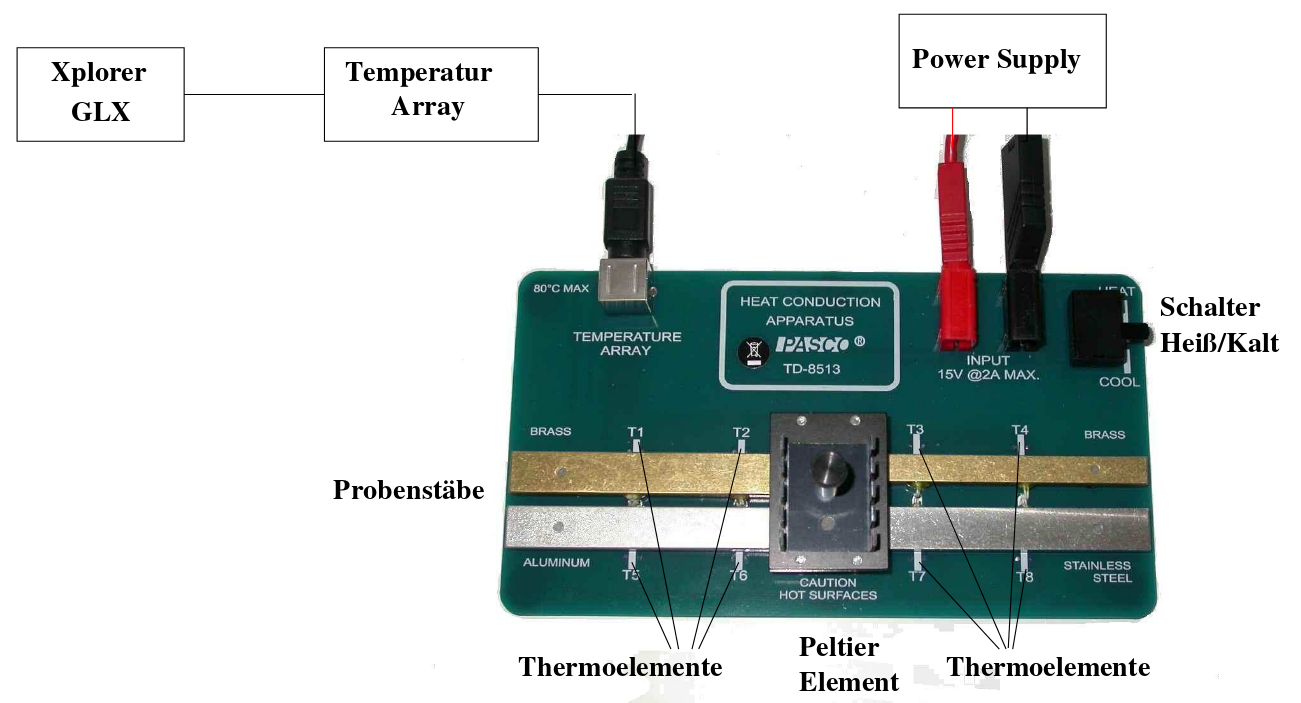
\includegraphics{content/aufbau.png}
\label{fig:aufbau}
\end{figure}
Dabei heizt das Peltierelement die vier Metallstäbe simultan und die Temperatur wird an 8 
verschiedenen Messpunkten, je zwei pro Stab, mithilfe vom Thermoelementen gemessen. Die 
Messwerte werden über 

\subsection{Statische Methode}
\label{sec:statische Methode}


\subsection{Dynamische Methode}
\label{sec:dynamische Methode}


